% Options for packages loaded elsewhere
\PassOptionsToPackage{unicode}{hyperref}
\PassOptionsToPackage{hyphens}{url}
\PassOptionsToPackage{dvipsnames,svgnames,x11names}{xcolor}
%
\documentclass[
  letterpaper,
  DIV=11,
  numbers=noendperiod]{scrartcl}

\usepackage{amsmath,amssymb}
\usepackage{iftex}
\ifPDFTeX
  \usepackage[T1]{fontenc}
  \usepackage[utf8]{inputenc}
  \usepackage{textcomp} % provide euro and other symbols
\else % if luatex or xetex
  \usepackage{unicode-math}
  \defaultfontfeatures{Scale=MatchLowercase}
  \defaultfontfeatures[\rmfamily]{Ligatures=TeX,Scale=1}
\fi
\usepackage{lmodern}
\ifPDFTeX\else  
    % xetex/luatex font selection
\fi
% Use upquote if available, for straight quotes in verbatim environments
\IfFileExists{upquote.sty}{\usepackage{upquote}}{}
\IfFileExists{microtype.sty}{% use microtype if available
  \usepackage[]{microtype}
  \UseMicrotypeSet[protrusion]{basicmath} % disable protrusion for tt fonts
}{}
\makeatletter
\@ifundefined{KOMAClassName}{% if non-KOMA class
  \IfFileExists{parskip.sty}{%
    \usepackage{parskip}
  }{% else
    \setlength{\parindent}{0pt}
    \setlength{\parskip}{6pt plus 2pt minus 1pt}}
}{% if KOMA class
  \KOMAoptions{parskip=half}}
\makeatother
\usepackage{xcolor}
\setlength{\emergencystretch}{3em} % prevent overfull lines
\setcounter{secnumdepth}{-\maxdimen} % remove section numbering
% Make \paragraph and \subparagraph free-standing
\ifx\paragraph\undefined\else
  \let\oldparagraph\paragraph
  \renewcommand{\paragraph}[1]{\oldparagraph{#1}\mbox{}}
\fi
\ifx\subparagraph\undefined\else
  \let\oldsubparagraph\subparagraph
  \renewcommand{\subparagraph}[1]{\oldsubparagraph{#1}\mbox{}}
\fi


\providecommand{\tightlist}{%
  \setlength{\itemsep}{0pt}\setlength{\parskip}{0pt}}\usepackage{longtable,booktabs,array}
\usepackage{calc} % for calculating minipage widths
% Correct order of tables after \paragraph or \subparagraph
\usepackage{etoolbox}
\makeatletter
\patchcmd\longtable{\par}{\if@noskipsec\mbox{}\fi\par}{}{}
\makeatother
% Allow footnotes in longtable head/foot
\IfFileExists{footnotehyper.sty}{\usepackage{footnotehyper}}{\usepackage{footnote}}
\makesavenoteenv{longtable}
\usepackage{graphicx}
\makeatletter
\def\maxwidth{\ifdim\Gin@nat@width>\linewidth\linewidth\else\Gin@nat@width\fi}
\def\maxheight{\ifdim\Gin@nat@height>\textheight\textheight\else\Gin@nat@height\fi}
\makeatother
% Scale images if necessary, so that they will not overflow the page
% margins by default, and it is still possible to overwrite the defaults
% using explicit options in \includegraphics[width, height, ...]{}
\setkeys{Gin}{width=\maxwidth,height=\maxheight,keepaspectratio}
% Set default figure placement to htbp
\makeatletter
\def\fps@figure{htbp}
\makeatother

\KOMAoption{captions}{tableheading}
\makeatletter
\makeatother
\makeatletter
\makeatother
\makeatletter
\@ifpackageloaded{caption}{}{\usepackage{caption}}
\AtBeginDocument{%
\ifdefined\contentsname
  \renewcommand*\contentsname{Indice}
\else
  \newcommand\contentsname{Indice}
\fi
\ifdefined\listfigurename
  \renewcommand*\listfigurename{Elenco delle Figure}
\else
  \newcommand\listfigurename{Elenco delle Figure}
\fi
\ifdefined\listtablename
  \renewcommand*\listtablename{Elenco delle Tabelle}
\else
  \newcommand\listtablename{Elenco delle Tabelle}
\fi
\ifdefined\figurename
  \renewcommand*\figurename{Figura}
\else
  \newcommand\figurename{Figura}
\fi
\ifdefined\tablename
  \renewcommand*\tablename{Tabella}
\else
  \newcommand\tablename{Tabella}
\fi
}
\@ifpackageloaded{float}{}{\usepackage{float}}
\floatstyle{ruled}
\@ifundefined{c@chapter}{\newfloat{codelisting}{h}{lop}}{\newfloat{codelisting}{h}{lop}[chapter]}
\floatname{codelisting}{Lista}
\newcommand*\listoflistings{\listof{codelisting}{Elenco degli Elenchi}}
\makeatother
\makeatletter
\@ifpackageloaded{caption}{}{\usepackage{caption}}
\@ifpackageloaded{subcaption}{}{\usepackage{subcaption}}
\makeatother
\makeatletter
\@ifpackageloaded{tcolorbox}{}{\usepackage[skins,breakable]{tcolorbox}}
\makeatother
\makeatletter
\@ifundefined{shadecolor}{\definecolor{shadecolor}{rgb}{.97, .97, .97}}
\makeatother
\makeatletter
\makeatother
\makeatletter
\makeatother
\ifLuaTeX
\usepackage[bidi=basic]{babel}
\else
\usepackage[bidi=default]{babel}
\fi
\babelprovide[main,import]{italian}
% get rid of language-specific shorthands (see #6817):
\let\LanguageShortHands\languageshorthands
\def\languageshorthands#1{}
\ifLuaTeX
  \usepackage{selnolig}  % disable illegal ligatures
\fi
\IfFileExists{bookmark.sty}{\usepackage{bookmark}}{\usepackage{hyperref}}
\IfFileExists{xurl.sty}{\usepackage{xurl}}{} % add URL line breaks if available
\urlstyle{same} % disable monospaced font for URLs
\hypersetup{
  pdftitle={Intorno al campanile di San Rocco},
  pdfauthor={Claudio Comandini},
  pdflang={it},
  colorlinks=true,
  linkcolor={blue},
  filecolor={Maroon},
  citecolor={Blue},
  urlcolor={Blue},
  pdfcreator={LaTeX via pandoc}}

\title{Intorno al campanile di San Rocco}
\author{Claudio Comandini}
\date{16 agosto 2024}

\begin{document}
\maketitle
\begin{abstract}
Nascita, sviluppo e prospettive di una città a partire dal suo monumento
più antico
\end{abstract}
\ifdefined\Shaded\renewenvironment{Shaded}{\begin{tcolorbox}[interior hidden, boxrule=0pt, breakable, frame hidden, borderline west={3pt}{0pt}{shadecolor}, enhanced, sharp corners]}{\end{tcolorbox}}\fi

\begin{figure}

{\centering 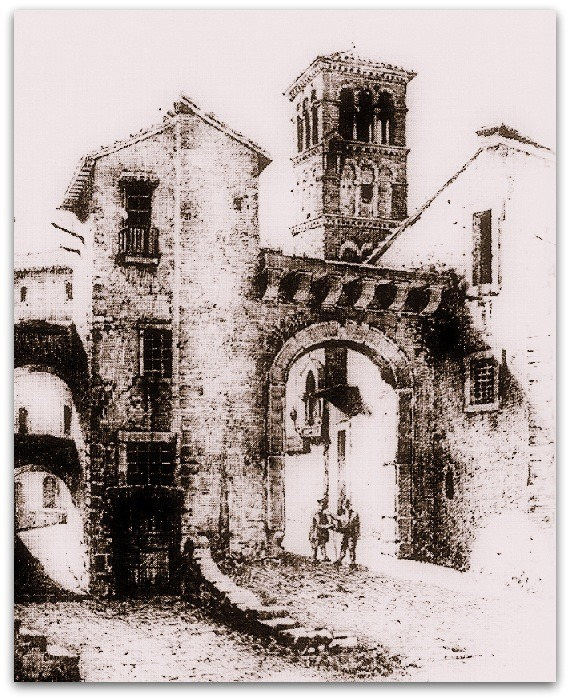
\includegraphics{../../images/2024/san_rocco/1CampanileSRoccoPortaCapestrano.jpg}

}

\caption{\emph{Campanile di S. Rocco e Porta Caperchiano, 1850 ca.}}

\end{figure}

\emph{Nascita, sviluppo e prospettive di una città a partire dal suo
monumento più antico.}

\hypertarget{in-vivarium}{%
\subsection{\texorpdfstring{1. \emph{In
Vivarium}}{1. In Vivarium}}\label{in-vivarium}}

La chiesa di S. Maria in \emph{«locus qui vocatur Frascata»} è ancora
oggi sulla piazza che porta il nome di S. Rocco, un po' spostata sulla
destra di chi guarda rispetto alla fontana e alla Rocca. La sua prima
menzione documentale compare sul Liber Pontificalis nell'876, insieme
alle chiese di S. Sebastiano, in seguito anche ospedale e quindi
cimitero, non più esistente dagli anni cinquanta del novecento, che
costeggiando il tratto urbano della Via Tuscolana era sul sito
dell'attuale scuola media (ora presso Via Domenico Seghetti), e di S.
Vincenzo, la cui collocazione è ipotizzabile dove venne eretta la chiesa
delle Scuole Pie, nella parte alta del tracciato urbano superiore della
via Tuscolana (lungo l'attuale Corso Italia). Nonostante alcune
inevitabili incertezze, per cui S. Maria e S. Sebastiano potrebbero
scambiarsi di posto e S. Vincenzo non ha effettivamente lasciato traccia
alcuna, questa è la ripartizione più plausibile. L'ultimo quarto
dell'800 è caratterizzato dalla dissoluzione dell'impero carolingio,
diviso in tre tronconi dei quali l'Italia settentrionale e centrale
occupano la parte più bassa di quello mediano, detto Lotaringia, il
quale a livello territoriale risulta particolarmente instabile. La
penisola è soggetta a numerose incursioni saracene, il ruolo universale
di Roma è minato dai conflitti con Bisanzio su questioni teologiche e da
quelli con la Germania sul ruolo imperiale nell'elezione del pontefice.
A Roma nel 901 la parcellizzazione dei feudi porta all'affermazione di
Teofilatto, ``\emph{iudex dativus}'', intendente di finanza con poteri
militari, capostipite della
\href{2012-05-10-possedimenti-memorie-tuscolo-comandini.html}{potente
casata tuscolana}. A ciò si accompagna il fenomeno
dell\emph{'incastellamento}, che concentra gli abitati nei fortilizi più
elevati.

Durante il lungo periodo segnato dall'influenza tuscolana, Frascati non
riceve nessuna menzione sui documenti, e torna successivamente alla
distruzione della città di Tuscolo con la denominazione di
\emph{castrum} nelle bolle di Innocenzo III dei Conti di Segni (1200),
Gregorio IX dei Conti di Segni (1228) e Innocenzo IV dei Conti di
Lavagna (1244) come S. Maria «\emph{in Frascata}», località indicata
quale fondo destinato ad uliveto; il nome deriva dalla presenza di
``\emph{frasche}'' e legna da ardere e, vista la data della prima
menzione, non hanno alcun senso le popolari attribuzioni relative alla
copertura delle rovine con tali frasche da parte degli scampati da
Tuscolo. Piuttosto, quanto va rimarcato è come i tre poteri il cui
compromesso si è basato sulla
\href{2016-09-07-8-settembre-frascati-tuscolo-comandini.html}{distruzione
dell'antica città} si spartiscono il bottino: a Roma si consolida il
Comune, l'impero domina anche nel meridione, il papato rilancia ogni sua
prerogativa. Nel territorio della Campagna Romana si accrescono i centri
che derivano dalla dispersione dell'immenso feudo tuscolano, del quale i
Castelli romani sono soltanto una parte e dei quali Frascati è il più
noto e centrale, tanto per la prossimità a Roma quanto per il ruolo nei
traffici locali e verso il meridione. La storia fa comprendere quanto la
località sia sempre stata terreno di battaglia tra poteri diversi; il
presente ricorda quanto necessiti di ricordarsi di sé.

\begin{figure}

{\centering 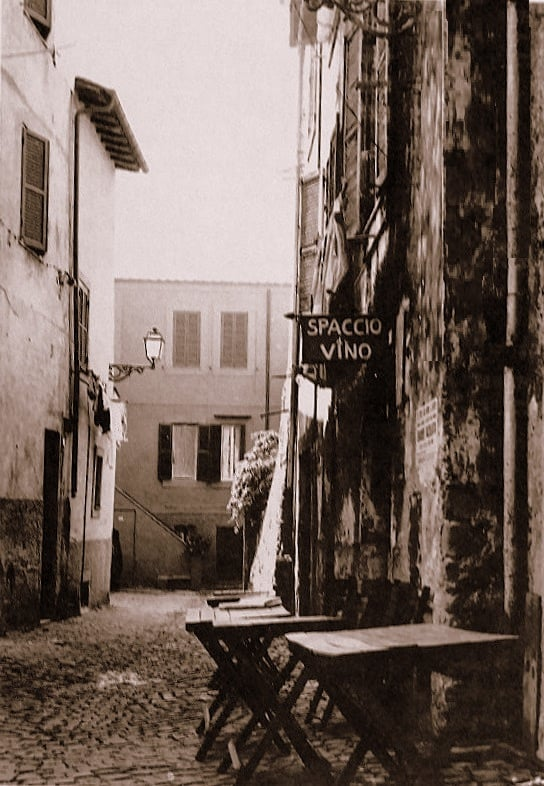
\includegraphics{../../images/2024/san_rocco/2matone.jpg}

}

\caption{\emph{Osteria del Dindolo al Matone,ca. 1980}}

\end{figure}

In un periodo in cui Tuscolo era ancora esistente, viene citata nei
documenti la piazza più antica di Frascati, piuttosto piccola e
nascosta, non distante dalla chiesa di Santa Maria in Vivario: la piazza
del Matone, sulla quale si affaccia un lavatoio pubblico chiuso
all'utenza dal 1983. Infatti, una Bolla del 1116 emanata dal pontefice
Pasquale II Raineri di Bleda menziona l'area del Matone. Il nome deriva
dal colle su cui la piazzetta poggia, e appartiene
all'\href{2016-12-31-momenti-fine-comandini.html\#parus\%C3\%ACa-unica-via}{Abbazia
Greca di Grottaferrata}; laddove il documento è reputato di dubbia
autenticità, risale al 1465, probabile anno di realizzazione del
lavatoio, il Regesto stilato dal cardinal
\href{2014-04-29-strade-fener-comandini.html\#partire}{Bessarione}, che
ne conferma nome e attribuzione, questa comunque da tempo decaduta.

Bessarione, esule di una Bisanzio ormai conquistata dai Turchi, è il
primo egumeno dell'Abbazia ed è inoltre vescovo della diocesi
suburbicaria, che in pratica significa extraurbana, denominata Labico
Quintanense, che ha ricevuto già diverse sedi, tra le quali Tuscolo e,
dopo la distruzione dell'antica città, Santa Maria in Monasterio
sull'Esquilino presso la Domus Aurea. Il coltissimo cardinale, esponente
del neoplatonismo, esercita le sue cariche mentre è pontefice
l'altrettanto erudito Pio II Piccolomini, ad un tempo il primo a
interessarsi alle rovine di Tuscolo e il primo a dotare Frascati di un
impianto urbano, stilato sul modello della città ideale già realizzato a
Pienza. Il nucleo del Matone, dove occupa l'area in cui le antiche mura
si risolvono nella cortina delle case, risulta limitrofo al tratto della
via Tuscolana che lo lambisce dall'attuale Via Ludovico Micara,
oltrepassando le Scalette di Porta Granara, nell'epoca che ci interessa
soltanto una salita in terra piuttosto ripida, che fiancheggia il dazio
e confluisce su uno degli estremi del \emph{castrum} (attuale via XX
Settembre); dalla parte opposta rispetto al Matone, si sviluppano i
rioni che compongono quello che chiamiamo quartiere di S. Rocco e che
nel dettaglio risulta piuttosto differenziato nelle parti.

Il nome \emph{vivarium} della chiesa deriva dalla vasca per la coltura
dei pesci della villa appartenuta al senatore Passieno Crispo e a sua
moglie Agrippina e infine a suo figlio Nerone, alimentata a suo tempo da
una sorgente probabilmente locata fuori porta presso l'attuale Chiesa
del Gesù, allora non esistente. Nei tempi antichi lo sviluppo della
villa e quindi della località segue per terrazzamenti successivi la
caduta delle acque, che trovano il loro punto di raccolta presso
l'attuale villa Campitelli nella cisterna di Galba, peraltro successore
di Nerone dopo il periodo dell'anarchia militare. Presso la zona di
\emph{Bagnara} (in via Luciano Manara, anticamente via di Sanguineto),
non lontano da un ninfeo romano scoperto nel 1854 ed erroneamente
attribuito a Lucullo dalla tipica fantasia popolare dei luoghi, venne
ritrovata una fistola, cioè una conduttura in piombo per l'acqua, con il
nome di Agrippina (custodita presso l'Orto Botanico di Roma).

La Villa di Lucullo, la prima attestata del territorio, la ritroviamo
fuori dal \emph{castrum}, e probabilmente si estendeva a partire dalla
zona dell'attuale parco comunale di Villa Torlonia. Invece, il
\emph{Mausoleo di Lucullo}, che fu anche monastero benedettino (ora
Torrione Micara), è incerto se sia appartenuta al grande console e
stratega romano, oppure ai Valerii Messalla, e si trova in un'area
piuttosto esterna al centro antico e quello moderno, sulla \emph{Via de'
Salé} (contrazione di Gerusalemme), diverticolo che conduce a S. Nilo
dal tratto in cui la via Tuscolana viene perlopiù chiamata via Romana.

\begin{figure}

{\centering 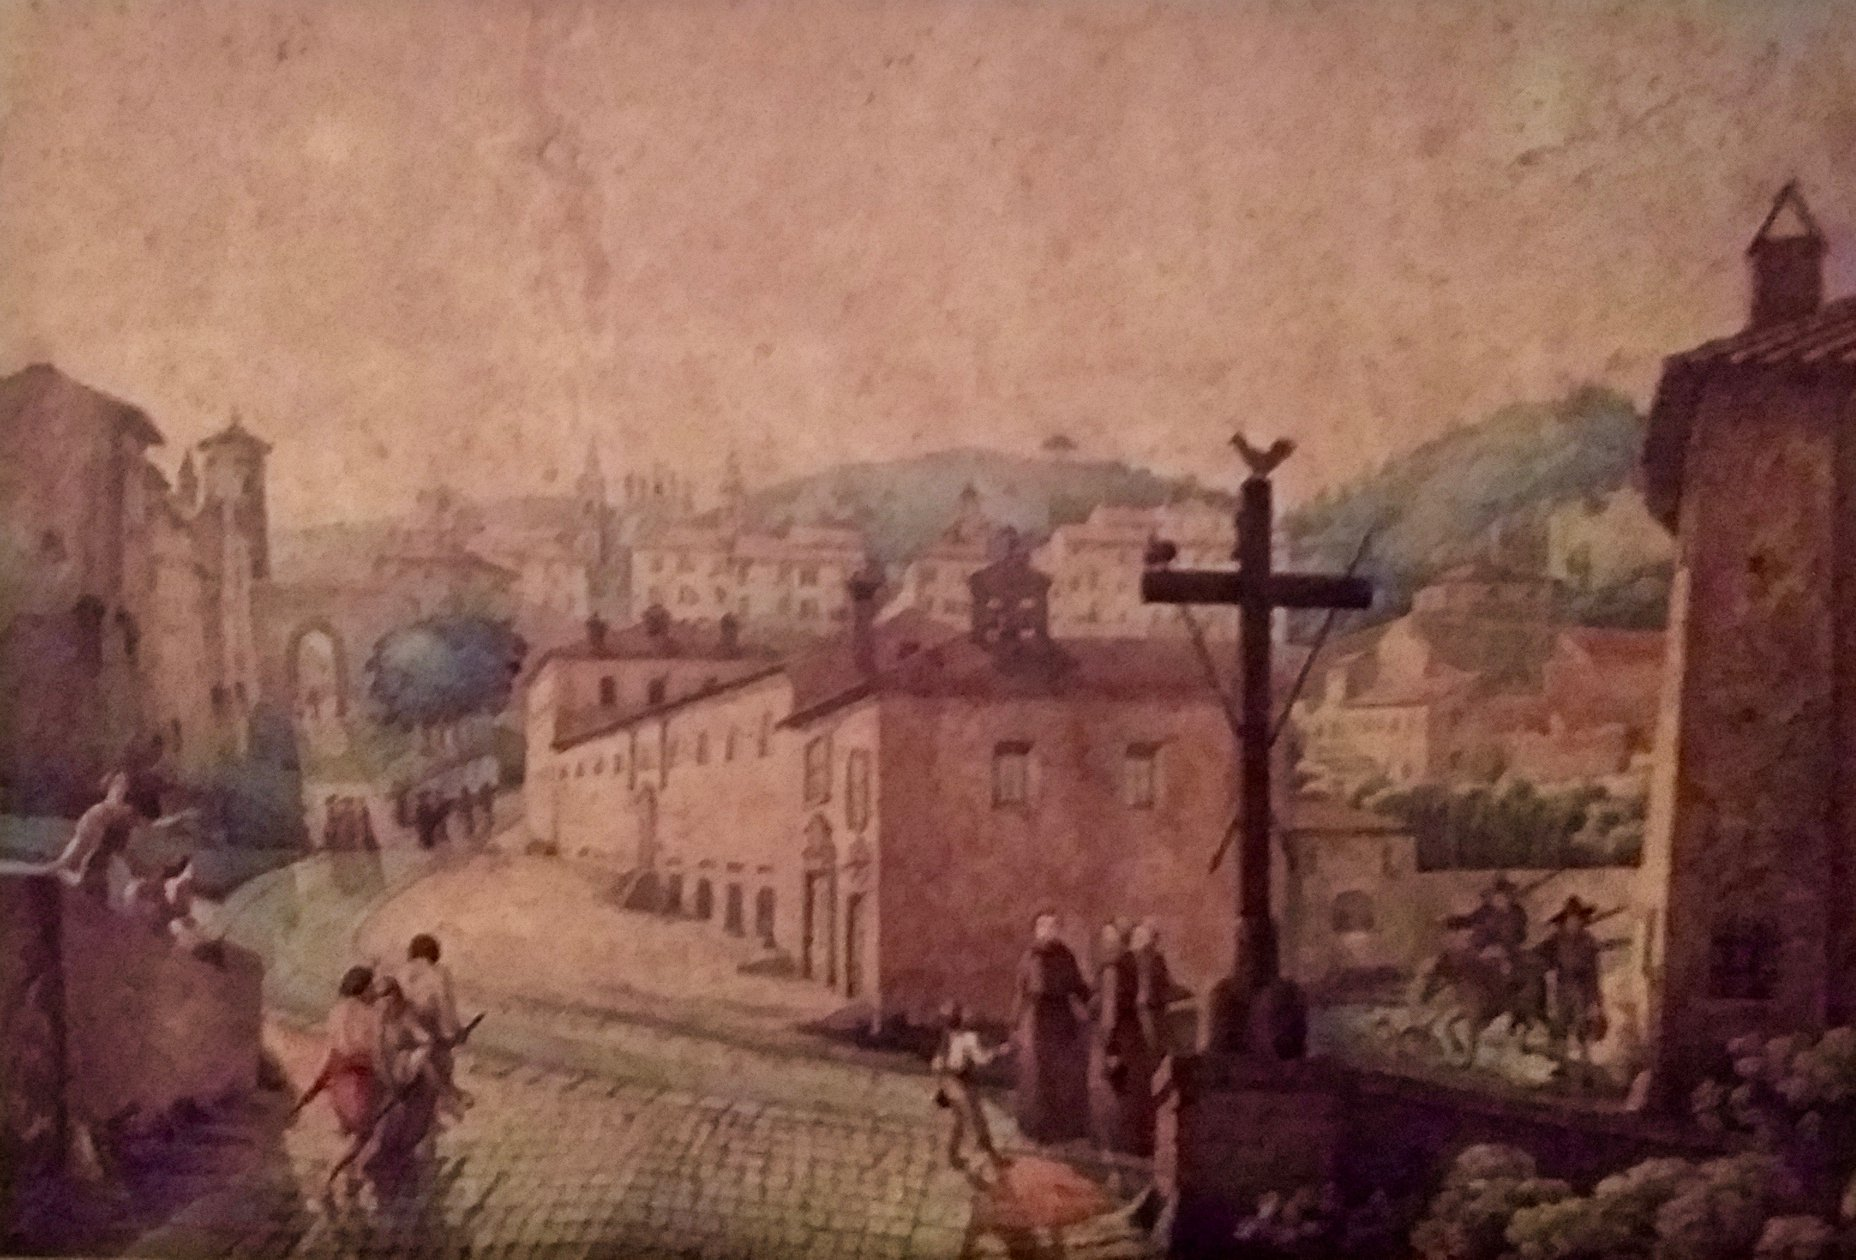
\includegraphics{../../images/2024/san_rocco/8largo-pentini.jpg}

}

\caption{\emph{Angelo Uggeri, Ospedale S. Sebastiano di Frascati, 1800
ca.}}

\end{figure}

Invece, presso l'allora \emph{Ospedale di S. Sebastiano}, venne
ritrovato un altro tratto di conduttura recante l'iscrizione del nome di
Nerone (conservato al Museo dell'Abbazia di Grottaferrata). È plausibile
che il controverso imperatore, in un panorama immenso che ancora oggi
incanta lo sguardo, abbia ammirato da qui l'incendio su Roma. Dopo la
sua sfortuna, il territorio diventa proprietà demaniale. Parte delle
rovine romane sottostanti sono tuttora accessibili dall'abside centrale
della chiesa, proprio dietro l'altare ricavato da un sepolcro
paleocristiano, mentre dalla sagrestia si accede alla cripta nei cui
pressi insiste il perimetro della chiesa primitiva del V sec.,
precedente quindi ogni fonte scritta conosciuta.

La chiesa viene ricostruita nel X sec., al tempo in cui la
\href{2012-05-10-possedimenti-memorie-tuscolo-comandini.html}{dinastia}
in seguito detta Tuscolana comincia ad espandersi, prima con Teoflilatto
e Teodora, poi con Marozia, quindi con il figlio di lei Alberico, e
infine con il figlio di questi, il pontefice Giovanni XII che,
incoronando imperatore il re sassone Ottone, rinnova l'istituto
imperiale. Domenico Seghetti e altri storici menzionano un rifacimento
ricevuto dalla chiesa nel 1296, e a detta del cardinal Ludovico Micara
in quell'anno Bonifacio VIII Caetani benedice la prima campana su quella
che deriva da una torre saracena e però esiste nella sua forma di
campanile in maniera accertata soltanto dal 1305. Per comprendere storia
e significato di questo primo monumento cittadino, sola testimonianza
medievale superstite, continuiamo a passeggiare nella storia e quindi
nelle sue vicinanze, lontani dal presente quanto basta per metterlo in
prospettiva e cercare di comprenderlo meglio.

\hypertarget{la-roma-dei-colonna-e-la-cattivituxe0-avignonese}{%
\subsection{2. La Roma dei Colonna e la cattività
avignonese}\label{la-roma-dei-colonna-e-la-cattivituxe0-avignonese}}

Alla fine del 1200 territorio e istituzioni sono segnate dal conflitto
tra papa Bonifacio VIII e l'illustre famiglia dei
\href{2015-12-15-marcantonio-colonna-frascati-comandini.html}{Colonna}.
La genealogia di questa, che si diffonde soprattutto nel Lazio e nel
Meridione, si collega per via di un fratello del pontefice
\href{2013-04-02-benedetto-ix-tuscolo-comandini.html}{Benedetto IX} ai
Conti di Tuscolo e di lì all'antichità e annovera nel blasone, per
costrutto ideologico che sia, oltre alla \emph{gens} Anicia e la
Mamilia, anche la Julia. Mantengono così un'impronta politica di
peculiare ispirazione romana, che tende alla protezione dell'Urbe pur
potendo condurre per le stesse prerogative alla sua destabilizzazione.
Il loro motto è \emph{Flecti Nescio}, e la loro capacità di resistere e
rilanciare è superiore ad ogni affondo possano ricevere. Dispongono di
centinaia di uomini e sono diffusi su tutto il territorio. Il loro
privilegio è quello di essere obbediti: se li incontri, devi fare quanto
ti dicono. Da parte sua, il cesaropapismo del pontefice tende a
riaffermare il ruolo accentratore della Chiesa mentre, con la
decapitazione di Corradino di Svevia da parte di Carlo D'Angiò del 1268,
l'impero si sta sfaldando e il contesto politico e sociale è ormai
prossimo a sganciarsi dalle strutture di potere feudali.

\begin{figure}

{\centering 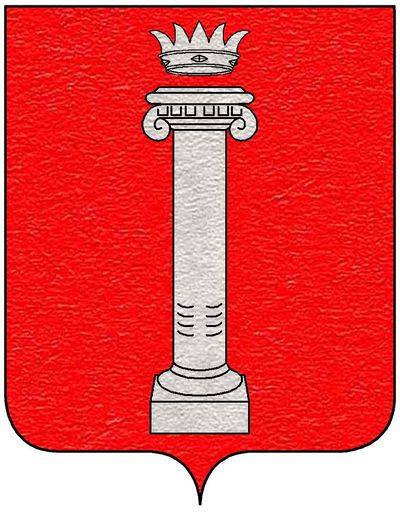
\includegraphics{../../images/2024/san_rocco/3Stemma_Colonna.jpg}

}

\caption{\emph{Stemma della famiglia Colonna}}

\end{figure}

Bonifacio VIII quindi deve combattere sovrani quali Ferdinando d'Aragona
di Sicilia, internamente alla Curia è contrastato dai cardinali Giacomo
e Pietro Colonna, a loro volta sostenuti dai Celestini e dai Francescani
Spirituali. Stefano il Vecchio, capostipite dei Colonna di Palestrina,
conte di Romagna e sposato a Guacerande di L'Isle-Jourdain in Guascogna,
compie nel maggio 1297 un'imboscata ai danni del pontefice presso Porta
Tiburtina, depredando un convoglio carico di duecentomila fiorini d'oro
atti ad acquistare un castello dai Frangipane. Conseguentemente, tutti i
Colonna vengono deposti e scomunicati, e costoro reagiscono con i
Manifesti di Lunghezza accusando il papa di elezioni illegali nonché di
essere responsabile della morte del suo predecessore Celestino V da
Morrone. I Colonna tentano la reintegrazione, ma nel dicembre 1297 una
vera e propria crociata porta a due anni d'assedio e quindi alla
distruzione di Palestrina, nonché alla confisca dei beni e alla
dispersione di quella che viene definita \emph{«dannata stirpe»},
esclusa persino dalle indulgenze giubilari del 1300.

Stefano il Vecchio e suo fratello Giacomo detto Sciarra (che vuol dire
rissa violenta), podestà di Narni, si ritirano presso la corte francese
preparando il terreno alla riscossa, che inizia a prendere luogo nel
1303 con lo \emph{Schiaffo di Anagni}, condannato nel canto XX del
\emph{Purgatorio} persino da
\href{2024-05-27-dante-islam-comandini.html}{Dante} che di Bonifacio era
avversario. Il pontefice, intenzionato a emanare una seconda scomunica
contro Filippo il Bello D'Angiò, viene imprigionato nel palazzo
pontificio di Anagni da Sciarra e dal cancelliere del re Guglielmo di
Nogareth che gli intima un processo, eppure riesce a fuggire. Il suo
successore Benedetto XI Boccassini annulla la scomunica contro i
Colonna, ma è comunque costretto a rifugiarsi a Perugia. Qui nel maggio
1305, dopo undici mesi di sede vacante, viene eletto Clemente V De Got,
due anni dopo coinvolto dal re francese nella persecuzione contro i
Templari. Nel 1309 il pontefice trasferisce la curia a Poitiers e nel
1313, pur ponendo sede ad Avignone, mantiene residenza nel feudo papale
di Carpentras.

\begin{figure}

{\centering 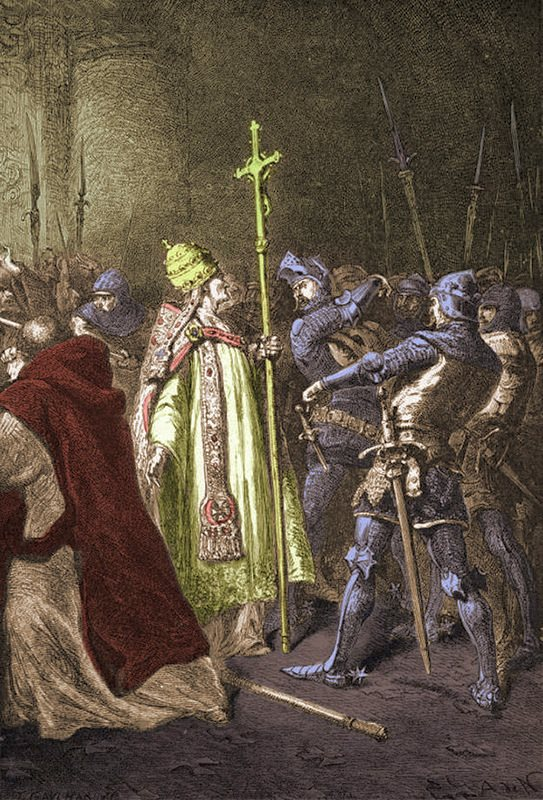
\includegraphics{../../images/2024/san_rocco/4AlphonsedeNeuville-SchiaffodiAnagni1883.jpg}

}

\caption{\emph{Alphonse de Neuville, Sciarra Colonna schiaffeggia
Bonifacio VIII (1883)}}

\end{figure}

Ai Colonna viene quindi accordato il recupero dei beni ed è concesso di
ricostruire Palestrina. Stefano il Vecchio esercita potere a Roma, nel
1313 al fianco del duca di Baviera e imperatore Enrico VII Wittelsbach.
Pur nella cruenza degli eventi, il suo comportamento appare esemplare:
rimane a fianco del sovrano anche quando questi attacca l'Urbe in modo
da poter esercitare quanto possibile garanzie, e pur favorendo pace
rifiuta l'investitura feudale che gli farebbe ottenere più potere. Nel
1328 Stefano sostiene il papa avignonese Giovanni XXII Duèze e il re di
Napoli Roberto D'Angiò, trovandosi sul campo avverso rispetto a Sciarra,
capitano del popolo romano, che da parte sua incorona come imperatore
Ludovico IV il Bavaro, il quale a sua volta nomina pontefice Niccolo V
Rainalducci. Si oppone loro Jacopo, uno dei figli di Stefano, che
provoca la fuga del Bavaro e dell'antipapa. Entrato nelle grazie del
legittimo pontefice, Jacopo è nominato vescovo di Lombes e intrattiene
rapporti con Francesco Petrarca.

Nel 1333 il tentativo di espansione del Bavaro verso Napoli provoca lo
scontro di Sciarra con gli Annibaldi che controllano il castello della
Molara, ultimo avamposto insieme
all'\href{2016-12-31-momenti-fine-comandini.html\#parus\%C3\%ACa-unica-via}{Abbazia
di San Nilo} di quello che fu Tuscolo. Il proposito viene abbandonato,
Sciarra muore in esilio, torna la pace tra i Colonna. Roma senza papa
continua ad essere travolta dalle consuete faide, in attesa di assistere
alla quasi messianica epopea di colui che, tra molte contraddizioni,
tenta di promuovere ordinamenti comunali definendosi quale ultimo
``\emph{tribuno del popolo}'', Cola di Rienzo. Inevitabilmente destinato
a scontrarsi con i Colonna, nel suo tentativo di riscossa del 1354
circonda di armate tutto il territorio attorno Palestrina, e a Frascati
concentra fanti e arcieri. Definitivamente caduto in disgrazia, viene
trucidato sul Campidoglio. Il suo cadavere squartato è lasciato appeso
davanti all'antico ingresso della Chiesa di S. Marcello in Via Lata, di
fronte alle abitazioni dei Colonna.

\hypertarget{breve-storia-di-una-chiesa}{%
\subsection{3. Breve storia di una
chiesa}\label{breve-storia-di-una-chiesa}}

Torniamo nel 1305 a Frascati dove, sotto l'autorità del Capitolo
Lateranense, la chiesa di S. Maria in Vivario riceve un campanile
romanico-romano rivestito in selce a tre ordini di trifore separati da
mensoline, simile a quello di S. Maria in Cosmedin presso la Bocca della
Verità a Roma. Nel 1478 Guillame D'Estouteville, normanno appartenente
alla famiglia reale francese, papa mancato e uomo più ricco della sua
epoca, da Sisto IV Della Rovere riceve Frascati come saldo per debiti; a
segno della sua munificenza lascia, oltre alla fontana ottogonale con
zampillo centrale in pietra sperone, detta anche \emph{lapis
tuscolanus}, otto figli nati da Girolama Tosti. La chiesa viene da lui
di nuovo consacrata nel 1495. Nel corso del secolo successivo nuovi
altari vengono realizzati dal governatore card. Giacomo Savelli.

Gli affreschi, dei quali molti nel tempo danneggiati dall'umidità e
quindi andati perduti, hanno attribuzione incerta. Romano Mergé ricorda
che vi lavorò anche Francesco Caiazza, vissuto a Frascati nell'attuale
via dell'Olmo, morto sul patibolo per fatti di sangue nel 1486 e del
quale è sparita pure la lapide dedicatoria. L'affresco in stile
raffaellesco dell'abside della chiesa, che raffigura l'incoronazione
della Vergine Maria, appartiene probabilmente al periodo Colonna-Della
Rovere, e quindi al primo quarto del 1500. Leonello Razza segnala che
nel \emph{Libro del Camerlengo} nel 1581 sono annotati notevoli restauri
e nuove pitture opera di ``Messer Richardo pittore''. Nel 1592 si decide
di non inumare più i defunti nella cripta sottostante, portando così
allo stabilirsi del Cimitero presso l'Ospedale di S. Sebastiano. Nel
1636 viene consacrata come nuova cattedrale la chiesa di S. Pietro, già
operativa dal 1610, che eredita suppellettili della sede precedente.

Dopo i fasti del periodo che procede da Paolo III Farnese a Paolo V
Borghese, nel quale i papi vi risiedono, Frascati si sviluppa oltre il
nucleo antico. Nel 1650 la cerchia muraria viene allargata portandola
dall'attuale via Cairoli a fronte della nuova cattedrale, tagliando in
diagonale quella che oggi è piazza S. Pietro. Dopo la peste del 1656,
alla chiesa di S. Maria viene aggiunta una dedica a
\protect\hyperlink{0}{S. Rocco} grazie alla riscoperta degli affreschi
tardo quattrocenteschi, e quindi del periodo D'Estouteville che, secondo
un'iconografia consolidatasi già all'epoca di Martino V Colonna,
raffigurano lui e S. Sebastiano. Laddove al soldato romano Sebastiano
era dedicata un'altra chiesa già da tempi remoti, il nome più tipico
della chiesa e della piazza diventa quello di Rocco, il santo di
Montpellier di origine tuscolana amico degli appestati, sempre in
compagnia del cane che gli porta cibo. Nuove immagini del culto dei
santi vengono realizzate nel 1715 nella cappella loro dedicata, che
riceve nuove decorazioni di Pietro Gagliardi e Domenico Jannetti nel
1867. Nel 1765 il \protect\hyperlink{0}{Duca di York}, ultimo
discendente degli Stuart e cardinale, vescovo della città per oltre
quarant'anni, compie rifacimenti interni ed esterni. L'intero complesso
è oggetto di restauri e aggiunte nel 1878 e quindi nel 1958-1969.
Soltanto allora le dieci colonne in pietra sperone furono liberate dalle
coperture in calce, al tempo della peste usata per allontanarla.

\begin{figure}

{\centering 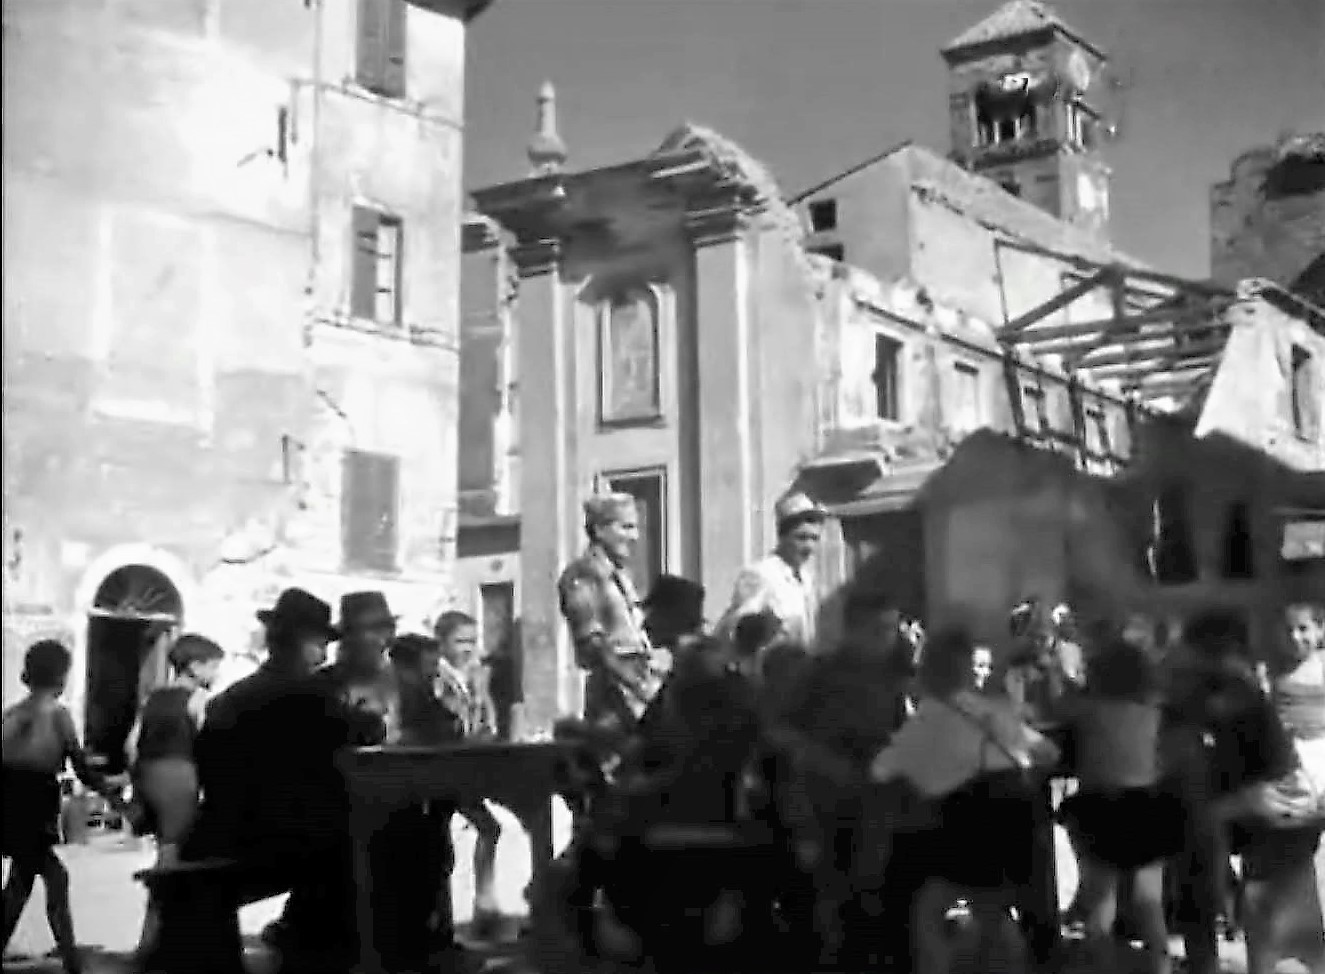
\includegraphics{../../images/2024/san_rocco/6san-rocco-bombe.jpg}

}

\caption{\emph{Bombardamenti presso la chiesa di S. Maria o S. Rocco a
Frascati, 8 settembre 1943}}

\end{figure}

I bombardamenti alleati
dell'\href{2016-09-07-8-settembre-frascati-tuscolo-comandini.html}{8
settembre 1943} colpisco la chiesa demolendone la parte più prossima
alla Rocca e operano chirurgicamente attorno al campanile isolandolo dai
palazzi cresciutigli intorno, attuando involontariamente un progetto del
1915. La muratura delle trifore impedisce al monumento di crollare.
L'orologio che vi era apposto dalla parte di Piazza Paolo III viene
spostato su uno dei campanili di S. Pietro. Oggi, a vederlo dalla
prospettiva della piazza, il campanile sembrerebbe appartenere al pur
valido negozio di generi alimentari della signora Mirella, e tutto il
tratto che lo unisce alla chiesa sottostante non è visibile in quanto
coperto da costruzioni di vario tipo e dal dislivello stradale. Sul lato
opposto, un pezzo di colonna romana rimane incastonato tra tali
costruzioni e l'angolo sinistro del campanile. Nella nicchia bassa vi
sono affreschi stratificati di autori ignoti; quello più in profondità
rendeva presente la figura del Figlio, quello in superficie quella della
Madre; ambedue sono stati recentemente coperti da un restauro che a
definirlo dilettantesco gli fai un complimento.

Nella piazza di S. Rocco nel 1969 la fontana ottogonale viene spostata
dalle adiacenze della Rocca e collocata al centro della piazza, dove era
stata originariamente posta nel 1480, concludendo così una lunga serie
di peregrinazione da un punto all'altro. Mergé segnala che nel 1769
Paolo Borghese principe Aldobrandini concesse al Duca di York l'acqua
per la Rocca; gli ampliamenti successivi delle condutture attraversano
tutta Frascati, arrivando presso la chiesa di S. Bonaventura (nel rione
anticamente detta \emph{Sanguineto}) partendo dalla zona del cosidetto
\emph{Sepolcro di Lucullo} (di era repubblicana ma non ben identificato,
nel 1598 spogliato di materiali utilizzati per S. Pietro e Villa
Aldobrandini). L'ottagono della fontana rimanda alla sovrapposizione tra
la Gerusalemme celeste e quella terrena, è combinazione dei punti
cardinali e quelli intermedi, nonché simbolo di resurrezione e vita
eterna. La lapide posta nella parte che guarda Roma ci ricorda che
``\emph{Ninphar haec domus}'': la fontana è casa di una ninfa. Le
fresche acque dell'Algidosia, che sgorgano presso la Molara, sono
protagoniste della cantata \emph{Circe} (1667) di Alessandro Stradella,
la cui prima esecuzione si svolge al Teatro delle Acque di Villa
Aldobrandini, nella quale vengono addirittura divinizzate.

\begin{figure}

{\centering 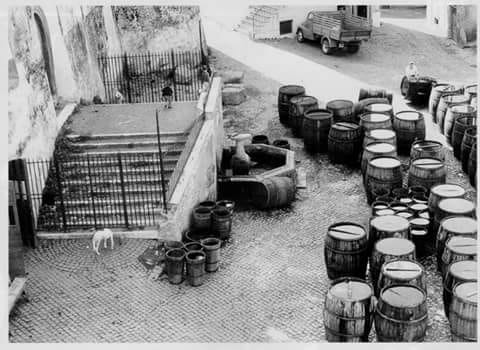
\includegraphics{../../images/2024/san_rocco/7san-rocco-botti.jpg}

}

\caption{\emph{Piazza S. Rocco al tempo della vendemmia, 1950 ca.}}

\end{figure}

Sul lato nord del campanile una lapide in marmo bianco dedicata alle
anime dei defunti ricorda con caratteri gotici fortemente abbreviati
alcune informazioni, invero piuttosto parziali e pasticciate. Segnala
che il campanile è stato realizzato il 26 aprile 1305, sotto Clemente V:
la scritta potrebbesi dire profetica, giacché il pontefice viene
ufficialmente eletto in maggio. Viene quindi la dedica ai defunti
``\emph{Andrea Madiss et Johannis Jordani}: a detta di Nibby, di
Santovetti e di Razza, l'indicazione potrebbe essere di due nomi, dei
quali almeno il secondo è tipico presso gli Orsini, storici rivali dei
Colonna, il cui antenato più illustre è papa Celestino III, tra i
responsabili della distruzione di Tuscolo. Da parte sua, Mergé
suggerisce si tratti di un unico nome, indicando nel secondo il genitore
del primo, il cui patronimico è riscontrabile in un notaio di casa
Colonna, i quali effettivamente si impongono a Frascati per una periodo
piuttosto rilevante, per quanto in maniera discontinua, per poi sparire
e tornare al massimo come governatori.

Osserviamone brevemente alcune fasi delle complesse e combattute vicende
nelle quali si intrecciano tra loro equilibri territoriali e rapporti di
potere che coinvolgono, oltre alle relazioni interne alla Stato
pontificio, anche quelle con altre potenze. I protagonisti delle
frequenti guerre civili appartengono più o meno sempre alle stesse
famiglie, ma le loro posizioni rispettive cambiano in ragione tanto
degli interessi consolidati quanto dei dissidi improvvisi. Nel 1420
Martino V, nativo di Gennazzano, ``capitale'' dello stato feudale dei
Colonna, porta a termine la cattività avignonese e lo scisma d'occidente
e, nello stabilirsi a Roma nel Palazzo dei SS. Apostoli, accompagna il
proprio rientro all'attribuzione dei territori della Chiesa ai suoi
congiunti; Frascati spetta, insieme a Molara, Montecompatri, Marino,
Rocca di Papa, Lariano, Genzano, Nemi e Ardea, al cardinal Prospero
figlio di Lorenzo. Tale controllo viene però perduto già sotto il
pontefice a seguire, il veneziano Eugenio IV Condulmer, che tenta di
contenere il potere dei Colonna ed è quindi nel 1434 da loro assediato e
quindi costretto a fuggire travestito da monaco fino a Civita
Castellana. Il papa si vendica tre anni dopo facendo distruggere,
un'altra volta, Palestrina, la cui fortezza viene ricostruita solo nel
1482, e quindi, coadiuvato dal condottiero Giovanni Vitelleschi, vengono
demolite Zagarolo e, parzialmente, il castello sulla via Latina già
dazio sotto i Conti di Tuscolo e al periodo tenuto dai Savelli (ora i
ruderi del castello di Borghetto sulla via Anagnina).

Invece, nel 1485, in occasione di un ennesimo scontro tra Colonna e
Orsini, Prospero Colonna figlio di Antonio, tra gli uomini d'arme
eminenti di un'epoca in cui la guerra era una delle belle arti, occupa
la Rocca di Frascati e rapisce Girolamo D'Estouteville, dal 1482
proprietario del feudo insieme al fratello Agostino. Sul lato
occidentale del campanile, non lontano da dove erano le fortificazioni,
è ancora visibile un'irregolarità della superficie che può ascriversi ad
un colpo di cannone. Gli Orsini quindi si uniscono a D'Estouteville, di
cui vengono rapiti anche moglie e figlio, e si combatte su tutto il
Lazio, da Nemi a Genazzano, da Marino a Bracciano; l'intervento di papa
Innocenzo VIII Cybo porta i Colonna, ma non gli Orsini, a rappacificarsi
con lui, e a Tivoli nel 1488 è pace anche tra Colonna e D'Eustoteville.
Le casate romane quindi si alleano nel contrastare il papa spagnolo
Alessandro VI Borgia.

\begin{figure}

{\centering 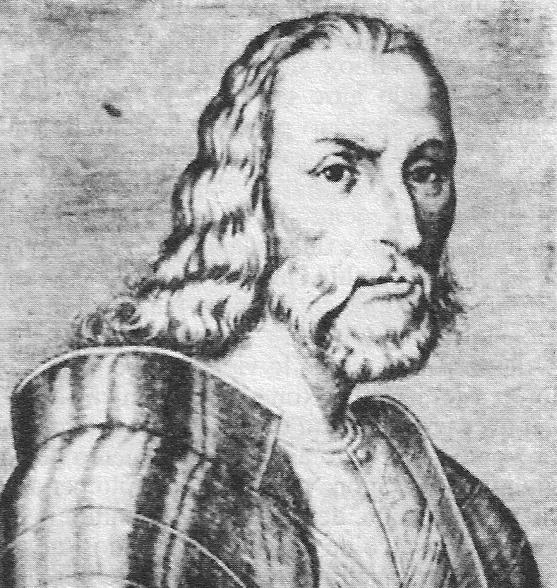
\includegraphics{../../images/2024/san_rocco/Prospero_Colonna.jpg}

}

\caption{\emph{Aliprando Caprioli, Ritratto di Prospero Colonna,
1596-1600}}

\end{figure}

Nel 1494 il re di Francia Carlo VIII di Valois discende in Italia
puntando a Napoli, dove è in ballo la successione al trono, e dà l'avvio
alle guerre d'Italia. I Colonna, insieme ad altri signori quali Ludovico
il Moro di Milano, gli si affiancano, vedendo nella sua calata,
conformemente al bieco e perenne particolarismo italico, l'occasione di
rilanciare e consolidare il proprio potere. Il pontefice, ostile al re
francese, requisisce i beni dei Colonna che stanno muovendogli sommossa.
Con un senso geografico piuttosto fantasioso, Frascati viene annessa al
ducato di Nepi, e la piccola Lucrezia figlia del papa potrebbe essere
così cresciuta, nell'isolamento sospettoso in cui i Borgia si tenevano,
oltre che in piazza Pizzo di Merlo a Roma, proprio nei luoghi tuscolani
che furono anche di Nerone. Alla nomina come Giulio II di Giuliano della
Rovere, deciso rivale di Borgia, i Colonna vengono reintegrati dei loro
beni. La nipote del pontefice Lucrezia della Rovere è data in sposa al
valoroso \protect\hyperlink{0}{Marcantonio I Colonna}, distintosi nella
battaglia che nel 1506 porta definitivamente Bologna nell'orbita romana.
Gli sposi ricevono congiuntamente in dote il feudo di Frascati, che nel
1515 viene fornito di uno Statuto cittadino.

Il Sacco di Roma del 1527, favorito dal focoso Pompeo Colonna, egumeno a
S. Nilo, fedelissimo dell'imperatore Carlo V d'Asburgo e da tempo
impegnato in una guerra personale con Clemente VII de' Medici, porta
l'Urbe in rovina, permettendo così una crescita di importanza di
Frascati, che scampa al massacro grazie alla protezione dei Colonna. Se
con il tempo la circostanza viene attribuita ad un intervento
soprannaturale determinato dall'immagine della Madonna di Capocroce
(all'incrocio dove oggi inizia la via Tuscolana), nel 1537 Frascati
passa alla Camera Apostolica, e quindi al diretto dominio papale,
attraverso complesse operazioni immobiliari mediate da Alessandro
Farnese, che fu a sua volta dalla parte dei Lanzichenecchi, il cui padre
è proprio il pontefice in carica Paolo III. La rivendicazione della
proprietà da parte di Ascanio Colonna non viene accolta, anche il
ricorso del ramo dei Colonna di Riofreddo viene cassato, così come
quello degli eredi D'Eustoteville, e nel 1538 il pontefice da
\emph{castrum} nomina Frascati quale \emph{civitas} attribuendogli la
sede vescovile suburbana che fu di Tuscolo-Labico Quintanense e il
titolo di cattedrale viene assegnato a S. Maria in Vivario. L'intensa
attività urbanistica, che inizia a svilupparsi verso la direttrice
sud-est, opposta a quella precedente, viene affidata a Sangallo il
Giovane, ed è ultimata la Rufinella, ora Falconieri, la prima delle
ville tuscolane volute dall'aristocrazia papale. La pace di
Cateau-Cambrésis del 1559 pone termine alle guerre d'Italia, portando
alla prevalenza asburgica sulla penisola; questo favorisce a Roma, il
cui potere è stato fortemente relativizzato dagli effetti della Riforma
protestante, di completare il Concilio di Trento. L'importanza di
Frascati, stabilizzatasi con un forte ancoraggio ai poteri romani, è
destinata a crescere.

\begin{figure}

{\centering 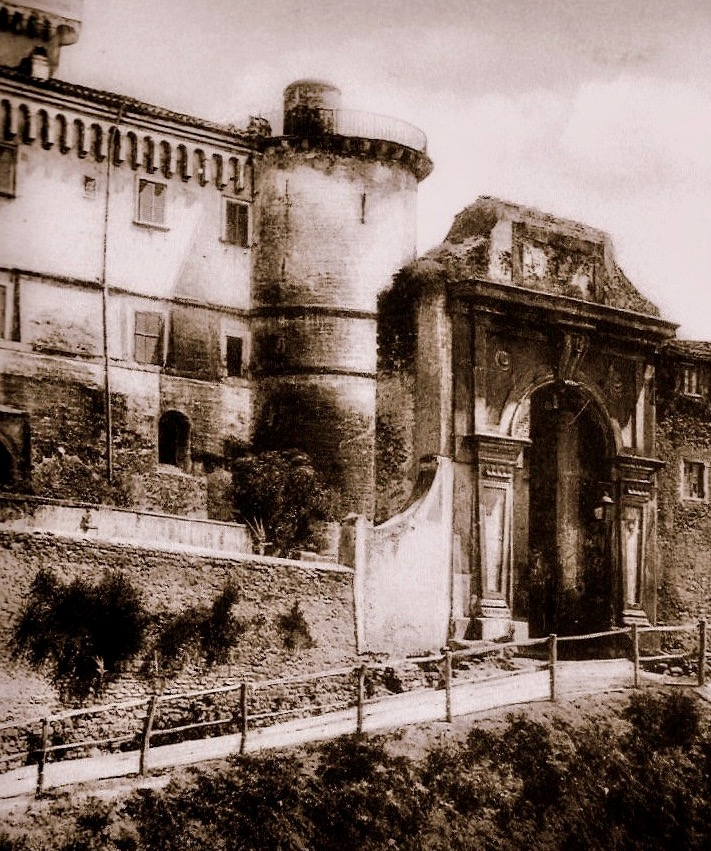
\includegraphics{../../images/2024/san_rocco/5porta_romana-antica.jpeg}

}

\caption{\emph{Porta Romana antica di Frascati, prima del 1888}}

\end{figure}

\hypertarget{in-giro-per-rioni}{%
\subsection{4. In giro per rioni}\label{in-giro-per-rioni}}

Il campanile rimane lì, dove ancora sta. Le maioliche circolari sulla
sua sommità, sette per ogni lato, cinque sopra e due sotto, conoscono
ancora i colori che ne videro le origini: rosso, giallo, verde e blu
variatamente assortiti. Torniamo quindi nei primi decenni del 1300, dove
sappiamo che i continui conflitti tra Colonna e Orsini e le lotte
intestine dentro le stesse famiglie nobiliari rendono Roma
ingovernabile. A breve verrà contesa tra diversi poteri anche Frascati,
ancora priva di fortificazioni e di modeste dimensioni che conta, come
si deduce dalla tassazione di dieci rubbie di sale al semestre imposta
dalla Camera Apostolica, circa un migliaio di abitanti.

Cerchiamo di ricostruire i rioni popolati da queste anime antiche nelle
strade di oggi. Le questioni sono rese complesse dai molteplici ed
enormi cambiamenti intercorsi, dai numerosi cambi di denominazione
nonché dagli impieghi diversi avuti da uno stesso nome. Molto è anche
andato perduto, ma oggi come ieri spesso la via indica il rione
adiacente. Il rione \emph{Vardesca}, che oggi fornisce nome a una via
spezzata in due tratti e ad una piccola piazza, è sul lato nord della
chiesa, ed è delimitato nella parte più ad est dal decumano romano,
attuale via dell'Olmo. Comprende l'area di Piazza Bambocci, il cui nome
deriva, in maniera simile pur se diversa rispetto alle
``\emph{grottesche}'' della Domus Aurea, dalle maschere rinvenute tra i
ruderi della villa di Nerone e usate come decorazione sulle case, che ha
come confine i bordi dell'attuale Piazza del Mercato, ai tempi non
esistente e delimitata da quella che poi venne chiamata Porta Spinetta.
Va segnalato che la denominazione di Piazza Bambocci prima del secondo
conflitto mondiale era attribuita all'attuale piazza Casini, e quella
che conosciamo oggi con tale nome era occupata da un agglomerato di
costruzioni basse e irregolari inframmezzate da viuzze dai nomi tipo Via
della Trippa e Via della Trippetta; come altri elementi, anche soltanto
nella zona troppi per venir qui nominati tutti, distrutti dalle
\href{2016-09-07-8-settembre-frascati-tuscolo-comandini.html}{bombe
angloamericane}.

Verso ovest, la Vardesca si estende dall'area che da \emph{via
Caperchiano}, scalinata che dall'arco di ingresso posto nei pressi del
campanile scendeva al borgo in basso, ricollegandosi con quella che era
chiamata \emph{Concia} e segnava un'area occupata da attività del
settore tessile. Da qui si incrocia la strada anticamente detta
\emph{Maremmana} (nel punto oggi alla confluenza tra Via Brigida
Pastorino e Via Gregoriana), che procede da via Sciadonna verso le
campagne. Nella parte più vicina alla chiesa, il rione era
caratterizzato dalla presenza di fortilizi medievali poi riadattati e
rovine romane, anche di epoca repubblicana, nel 1888 coperti dalla
realizzazione di via Regina Margherita, la cosiddetta ``\emph{Via
Penza}'', via pensile ideata dal Valadier che guarda verso il cimitero
moderno. Prima di ciò, era qui che scorreva l'antica via della Vardesca
(poi via di Saponara), il cui nome deriva, come ogni parola che
riguardano \emph{guardie} e corpi di guardia, dalla radice tedesca
\emph{qward}. Di fatto, gli attacchi militari venivano perlopiù da quel
versante, esposto al traffico della Labicana-Casilina, ed è oltre di
esso che si sono svolte le più importanti battaglie del territorio: nel
496 a.C. quella del Lago Regillo tra Lega latina e Repubblica romana, e
nel 1167 quella di Prataporci tra le truppe comunali e pontificie di
Roma contro quelle imperiali e tuscolane.

\begin{figure}

{\centering 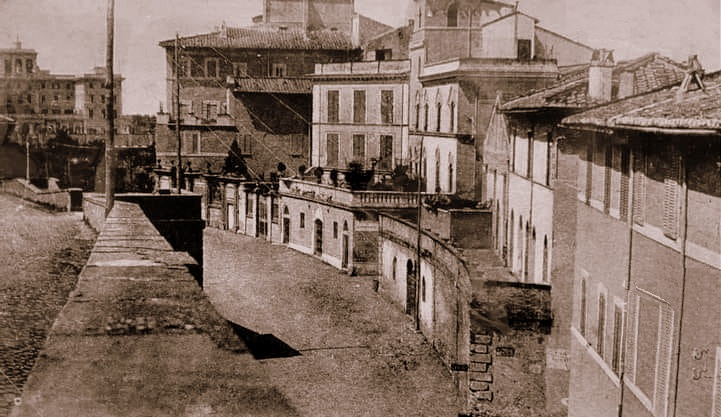
\includegraphics{../../images/2024/san_rocco/9via-borgo-san-rocco.jpg}

}

\caption{\emph{Via Borgo S. Rocco, prima del 1950}}

\end{figure}

\emph{Vallocchia} è nel livello più in basso, nell'attuale largo
Pentini, e accoglie il diverticolo che dalla Tuscolana conduceva a Porta
S. Rocco, il più antico ingresso della città. La porta venne abbattuta
per i lavori della via pensile insieme alle piccole abitazioni che la
fiancheggiavano e ad un tratto di mura che ancora portava lo stemma
Piccolomini. Per lungo tempo erroneamente attribuita al Vignola, la
possiamo immaginare collocata tra i due platani del terrazzamento
prospiciente la Rocca, la cui prospettiva definiva l'emiciclo
sottostante dell'abitato che caratterizzava quella che oggi chiamiamo
via Borgo S. Rocco.

\emph{Piazza del Mercato}, nella parte superiore della Rocca, doveva il
nome al mercato settimanale concessovi il giovedì, come citato nella
lapide del 1697 apposta su una colonna romana che si eleva sulla fontana
in pietra sperone con mascherone e vasca. La fontana è probabilmente la
prima pubblica della città, le cui acque provengono da Grottaferrata e
dall'acqua Mariana, conosciuta anche come Crabra; questa alimenta quello
nel 1122 deviato a favore di Roma, chiamato fiume Tuscolano da Cicerone
(la cui villa era o nei presso il sito dell'Abbazia, o nei dintorni di
Villa Falconieri). La colonna che sornonta la fontana era
originariamente posta all'inizio della discesa intitolata a
D'Estouteville, e i due monumenti vennero sovrapposti nel 1840.
Precedentemente la concessione di Paolo V del 1607 di tenere mercato
nelle mura cittadine, questo veniva effettuato nella parte esterna alle
mura e quindi nella succitata zona di incrocio tra via di Caperchiano e
la Vallocchia. Alla colonna si sovrappongono le chiavi papali dello
stemma cittadino deciso da Paolo III, al quale oggi la piazza è
dedicata, e quindi delle pignatte che rappresentano lo stemma di
Innocenzo XII Pignanelli sotto il cui pontificato vengono eretti i
monumenti, e il cui nome è ricordato insieme a quello del governatore
Carlo Colonna, nominato anche nella coeva facciata della cattedrale S.
Pietro.

\begin{figure}

{\centering 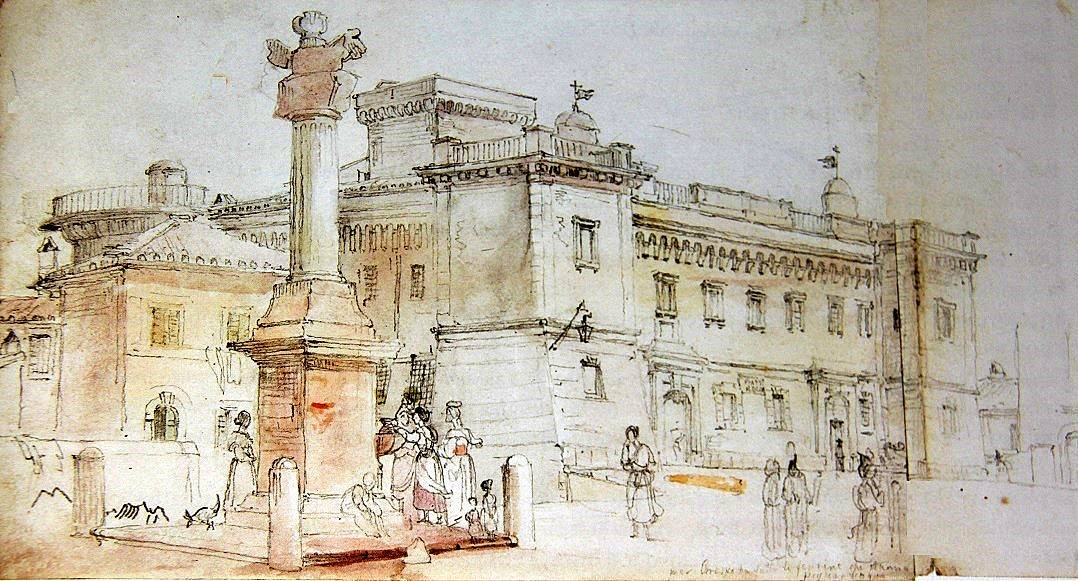
\includegraphics{../../images/2024/san_rocco/11rocca-fontana-superiore.jpg}

}

\caption{\emph{Veduta della piazza della Rocca di Frascati, 1840 ca.}}

\end{figure}

La Rocca rivela interventi che si sono succeduti nel tempo, da Pio II
Piccolomini a cui si deve la fondazione, al D'Estouteville che la
fortifica, ai vari passaggi dei Colonna, e allo stesso Paolo III che ne
aggiorna l'aspetto che dà sulla sua piazza riallestendo la stessa con
demolizioni e ricostruzioni mirate. Il
\href{https://grandtour.shop/posts/pages/2017-05-20-frascati-goethe-comandini.html}{Duca
di York} erige la torre in stile scozzese, ornata internamente dalle
tele affrescate del pittore polacco Taddeo Gunz, e dopo di lui
l'edificio viene appellato quale Palazzo vescovile; laddove dal 2023 la
sede vescovile è stata posta a Velletri, il piccolo castello deve
ricominciare a farsi chiamare \emph{Rocca} e va definitivamente
tematizzato quale cuore del centro storico. Da parte loro, fontana e
pertinenze, le cui prossimità sono molto frequentate a tutte le ore,
risultano piuttosto malmesse, danneggiate dall'incuria amministrativa e
dal vandalismo generico di chi ha piantato rampini e inciso sui
monumenti come se niente fosse, e al massimo ci ha messo un rubinetto
non pertinente al contesto.
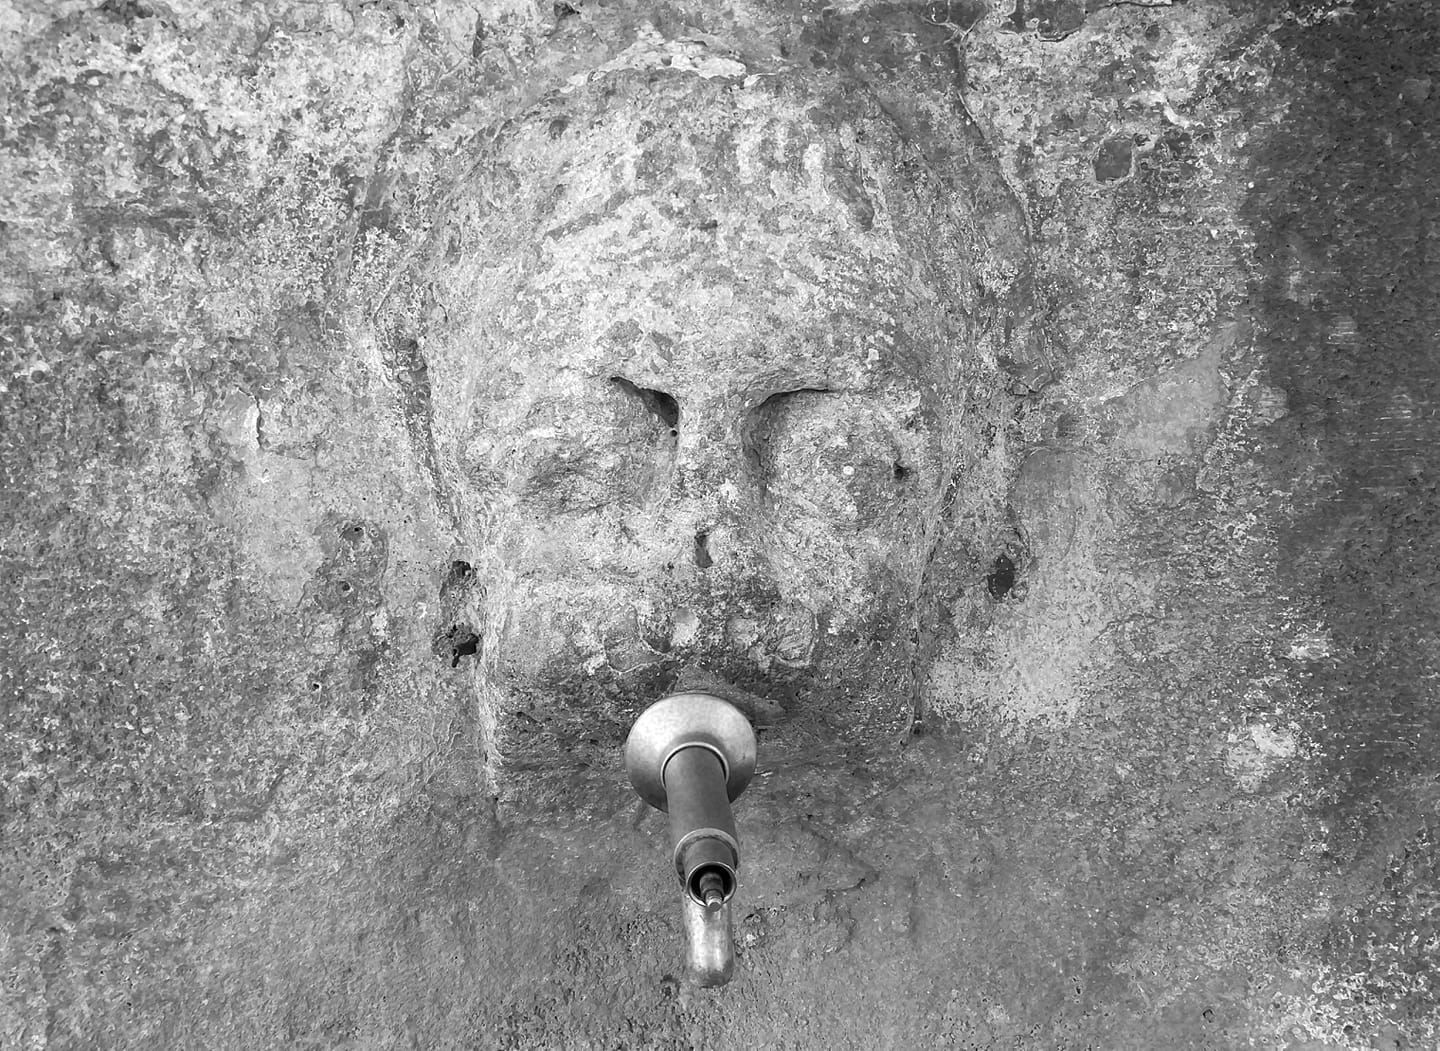
\includegraphics{../../images/2024/san_rocco/10mascherone.jpg}

Adiacente a tale piazza, quello che oggi chiamiamo largo duca di York,
già \emph{via delle Carceri}. Nella parte occidentale si elevava un
palazzo fatto costruire dal cardinal Giacomo Savelli, governatore di
Frascati, che nel 1553 diviene oggetto di una ribellione popolare a mano
armata, determinata da vessazioni eccessive in contrasto con lo Statuto
colonnese. Nel 1590 viene venduto alla Comunità che vi realizza il
secondo edificio comunale, successivo a quello del palazzo senza
fondamenta che attualmente a piazza Bambocci ospita il Forno Ceralli. La
centralità della zona favorisce la crescita del suo prestigio, e il
palazzo viene ampiamente ristrutturato nel 1771, affiancandosi così al
palazzo vescovile. Nel 1868 la sede comunale viene spostata a Palazzo
Botti, poi anche Casa del Fascio, quindi Tribunale, ora adibito a uffici
per servizi comunali, adiacente la cattedrale di S. Pietro. Palazzo
Savelli viene venduto alla Sede Apostolica, che vi stabilisce il Carcere
Giudiziario, sostituendosi al primo carcere che, come segnala la
sagomatura a ``\emph{mezzo litro}'' della grata in Via D'Estouteville,
era nei sotterranei della Rocca. Demolito dalle bombe
dell'\protect\hyperlink{0}{8 settembre}, prende il suo posto una brutta
palazzina di case popolari di proprietà comunale.

La zona, la cui rinascita è dovuta al lavoro delle attività lì presenti,
che caratterizzano in modo peculiare per quanto disordinato la movida
cittadina, ancora mantiene in modo incongruo il declassamento deciso dai
tempi in cui era sopratutto il carcere a caratterizzare l'area, senza
però mantenere il fascino del posto solitario lontano dalla pazza folla.
E, per quanto l'area possa offrire ad ognuno la sua ora d'aria e rancio
su misura, sembra incombere un oblio generale che svilisce i pur
notevoli potenziali e minimizza gli interventi necessari, aggravando le
difficoltà di gestire adeguatamente tanto il traffico locale quanto il
flusso turistico nonché la stessa abitabilità, lasciandoci in attesa
della cura che restituisca piena dignità storica e urbanistica a quanto
già da tempo ha prodotto città e conosciuto storia. E, mentre si
mantiene un irresponsabile conflitto tra residenti ed esercenti e i
visitatori pascolano distratti, si resta in attesa di interventi che
restituiscano pieno decoro all'area più centrale e tipica di un paese
che, oltre ad aver visibilmente smarrito la gloria di un tempo, sembra
piuttosto smarrito anche nel presente più ordinario. Nella parte
orientale del Largo, c'è poi il \protect\hyperlink{0}{Grand Tour
BookWineBar}, da cui ora vi scrivo: se passate, posso raccontarvi questa
e altre storie.

\begin{figure}

{\centering 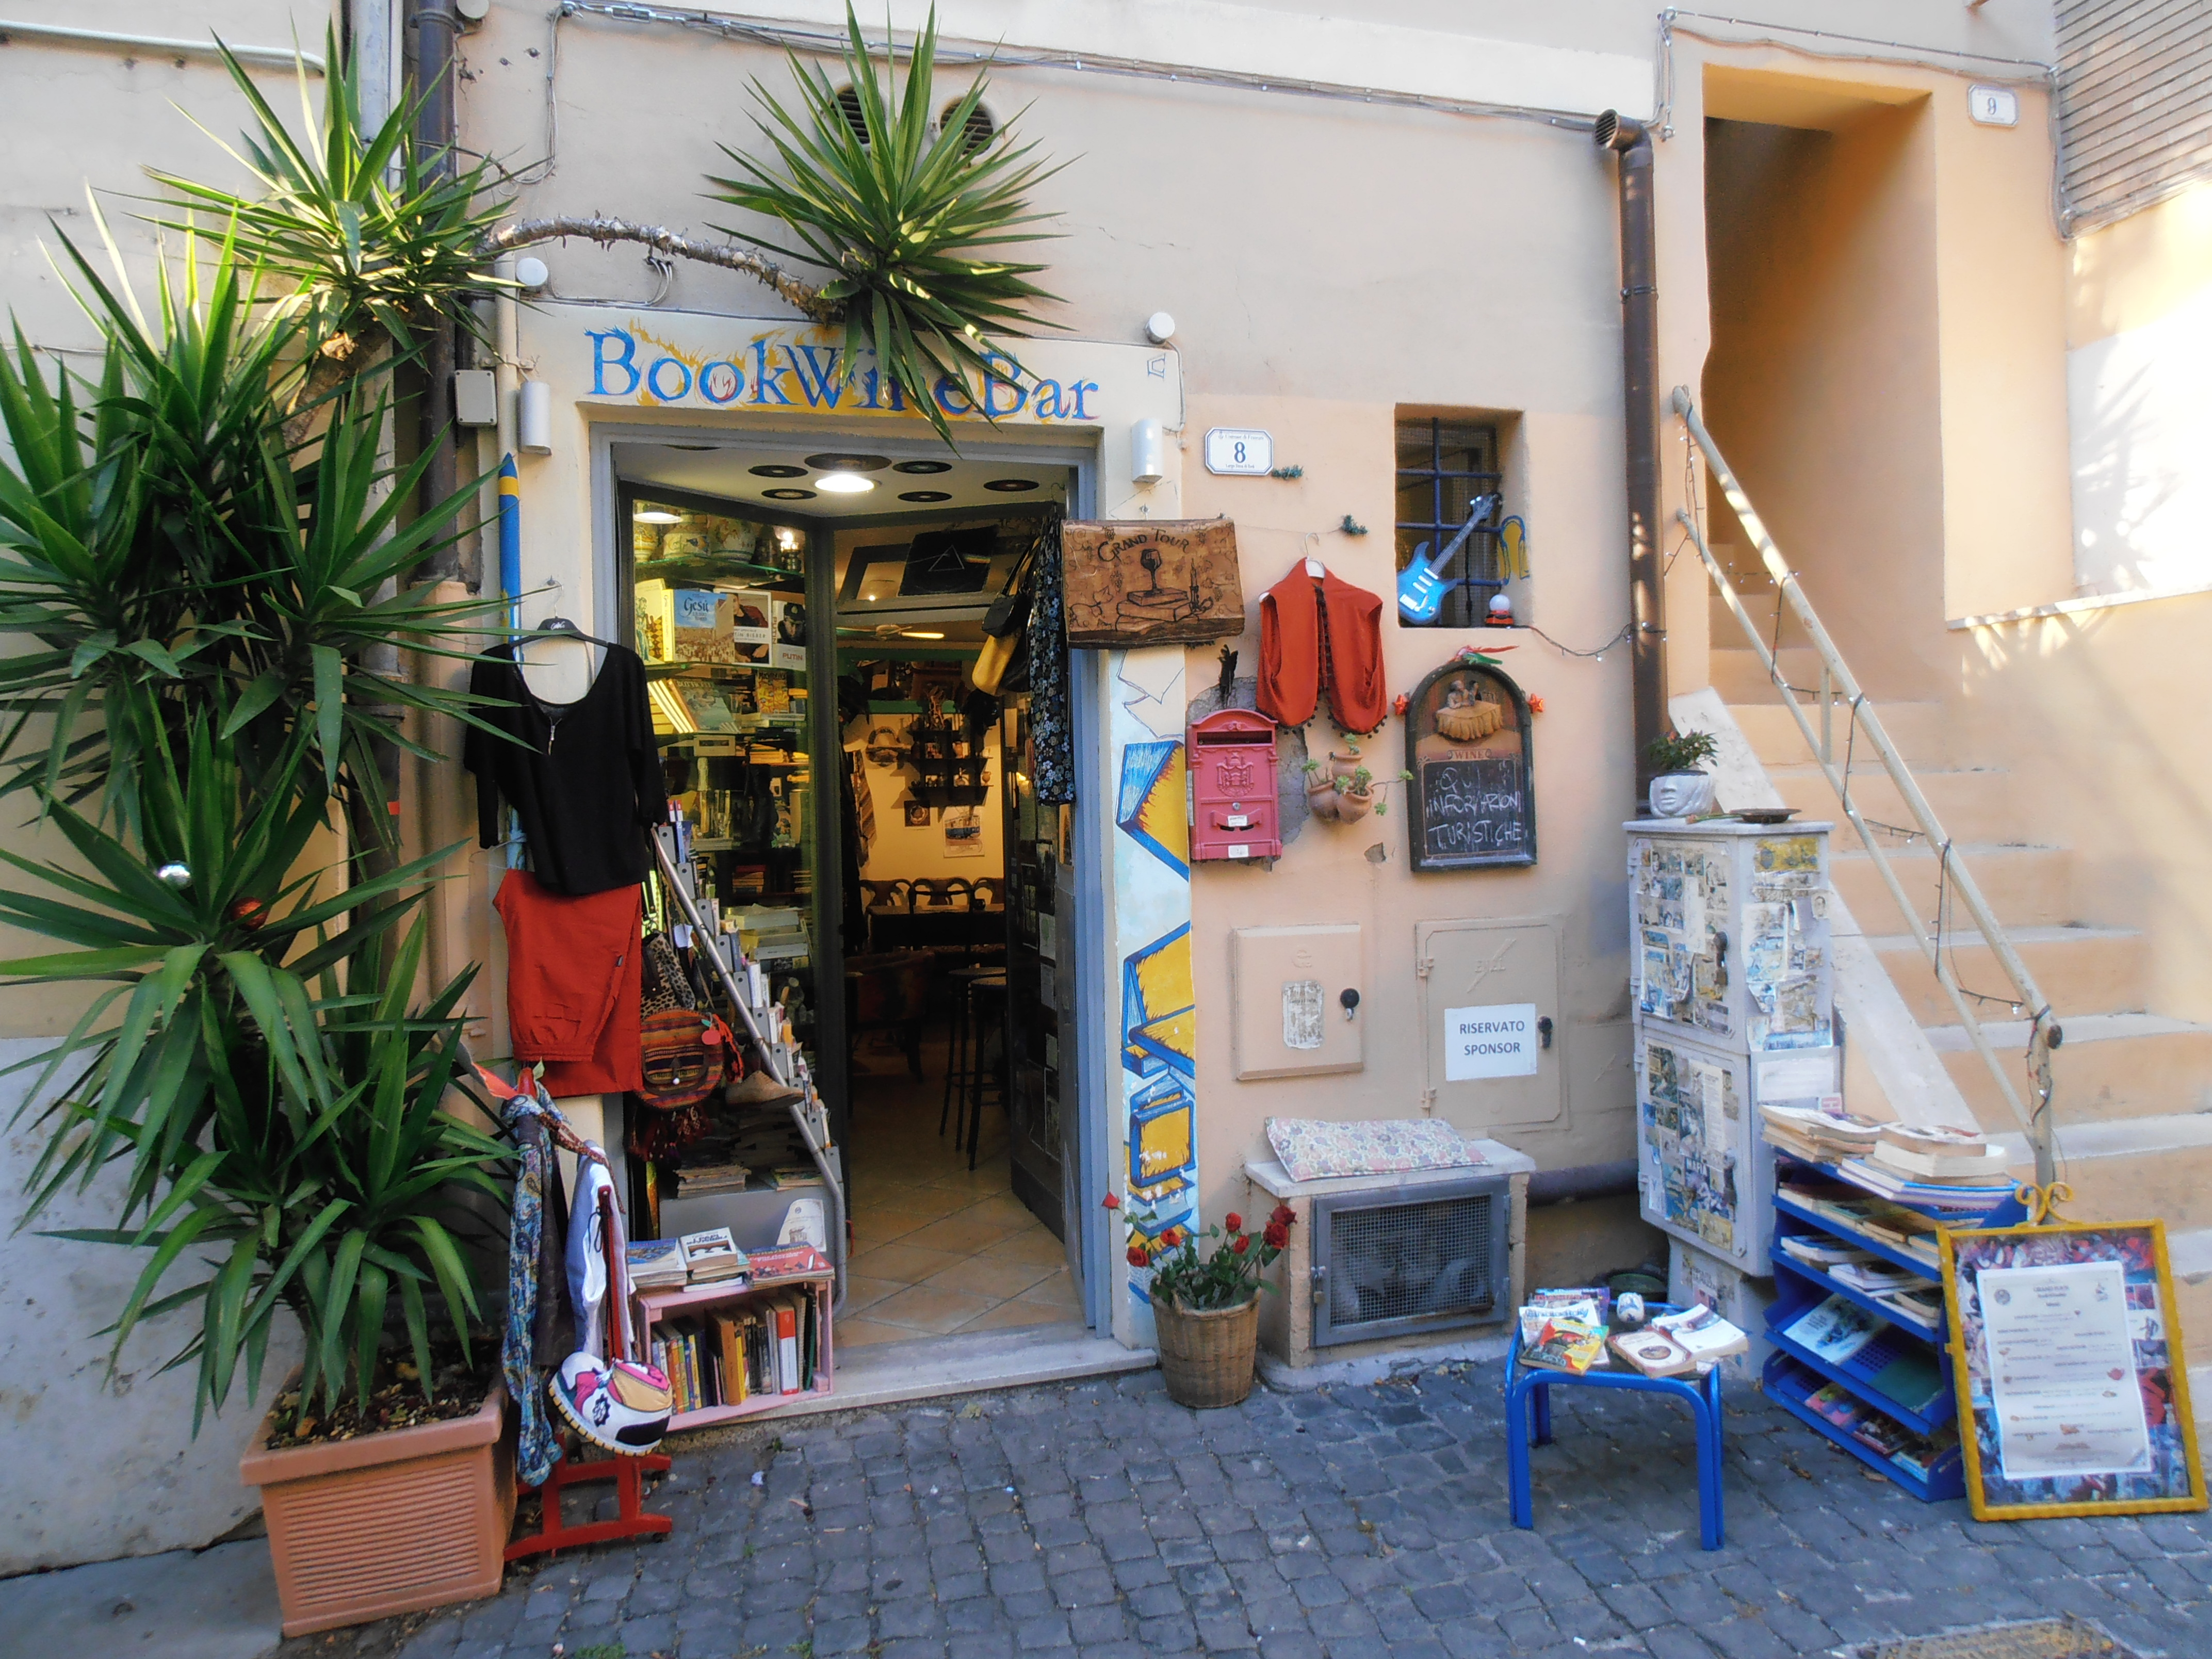
\includegraphics{../../images/immagini_bookwinebar/fuori1.JPG}

}

\caption{\emph{Grand Tour BookWineBar a Largo Duca di York, 2024}}

\end{figure}

\hypertarget{percorsi-in-ordine-cronologico}{%
\subsection{Percorsi (in ordine
cronologico)}\label{percorsi-in-ordine-cronologico}}

Domenico Barnaba Mattei, \emph{Memorie istoriche dell'antico Tuscolo,
oggi Frascati} {[}1711{]}, Forni 1979 {[}ristampa anastatica{]}.

Antonio Nibby, \emph{Analisi storico topografica antiquaria della carta
de' dintorni di Roma} - 3 voll. {[}1837{]}, Tipografia delle Belle Arti
1849 {[}seconda edizione{]}.

Ferdinand Gregorovius, \emph{Storia della città di Roma nel medioevo}
{[}1873{]}, Einaudi 1973.

Domenico Seghetti, \emph{Frascati nella natura, nella storia, nell'arte}
{[}1906{]}, Atesa 1986 {[}ristampa anastatica{]}.

Giuseppe Tomassetti, \emph{La Campagna romana} - 3 voll.\emph{,}
Loescher 1910.

Prospero Colonna, \emph{I Colonna dalle origini all'inizio del secolo
XIX}, Stabilimenti Poligrafici Alterocca-Terni 1927.

Vincenzo Celletti, \emph{I Colonna principi di Paliano}, Ceschina 1960.

Evaristo Dandini, \emph{Frascati nelle sue strade} {[}1962{]}, Cavour
Libri 2016 {[}aggiornato ai nuovi toponimi{]}.

Leonello Razza, \emph{S. Maria in Vivario. Vicende storiche dell'antica
cattedrale di Frascati}, Ed. Vivarium 1975.

Romano Mergé, \emph{Frascati sconosciuta}, Associazione Tuscolana «Amici
di Frascati» 1983.

Romano Mergé, \emph{Frascati nella realtà documentata} - vol.~I,
Associazione Tuscolana «Amici di Frascati» 1988.

Romano Mergé, \emph{Frascati nella realtà documentata} - vol.~II,
Associazione Tuscolana «Amici di Frascati» 1989.

Paolo Mascherucci, \emph{La diocesi suburbicaria di Frascati e i suoi
cardinali vescovi}, Associazione Tuscolana «Amici di Frascati» 1991.

R. Del Nero, M. B. Guerrieri Borsoi, I. Salvagni, C. Baldoni-L. Cemoli,
L\emph{'urbanizzazione della città di Frascati dal I sec.~ad oggi},
Associazione Tuscolana «Amici di Frascati» 2011.

\emph{Pubblicato in forma breve su «il Tuscolo» \#211, 15.12.2018.
Riveduto e ampliato.}



\end{document}
